\section{Introducere}

Aceasta lucrare prezinta implementarea unui predictor de ramificatii de tip
\textbf{Optimized GEometric History Length (OGEHL)} si integrarea sa in simulatorul
\textbf{SimpleScalar (simple-sim)}. Ca referinta de comparatie este folosit predictorul
hibrid de valori \textbf{Wang~'97}, pentru a ilustra diferentele
arhitecturale si functionale dintre cele doua abordari.

Structura lucrarii este urmatoarea: sectiunea~\ref{sec:simplescalar} descrie
simulatorul SimpleScalar, sectiunile~\ref{sec:ogehl} si~\ref{sec:wang} prezinta
cei doi predictori, sectiunea~\ref{sec:comparatie} ii compara, iar
sectiunea~\ref{sec:hw} detaliaza arhitectura hardware a OGEHL.

% -------------------------------------------------- SimpleScalar
\subsection{Simulatorul SimpleScalar}
\label{sec:simplescalar}

\textbf{SimpleScalar} este un set de instrumente care modeleaza un sistem de
calcul virtual format din CPU, ierarhia de cache si memoria principala.
Utilizand aceste instrumente, cercetatorii pot construi simulatoare pentru
programe reale care ruleaza pe o gama variata de procesoare moderne.
Pe langa simulatoare, pachetul include instrumente de vizualizare a
performantei, resurse pentru analiza statistica si infrastructura de depanare.
Instrumentele SimpleScalar sunt utilizate pe scara larga in cercetare si
educatie --- in anul 2000, mai mult de o treime dintre lucrarile publicate in
conferintele de top din arhitectura calculatoarelor au folosit SimpleScalar.

SimpleScalar poate simula arhitecturile \textbf{Alpha} si \textbf{PISA}
(Portable ISA). ISA-ul PISA este un set de instructiuni simplificat, similar
cu MIPS, destinat in principal scopului educational. Setul de instrumente
ruleaza binare compilate pentru aceste arhitecturi si le simuleaza pe unul
dintre mai multe modele de procesoare disponibile. Masina pe care ruleaza
SimpleScalar se numeste \textit{masina gazda} (Host), iar arhitectura
simulata se numeste \textit{tinta} (Target). Exista un cross-compiler GCC
pentru PISA, care creeaza iluzia ca instructiunile ruleaza pe o masina PISA
reala, desi ele sunt simulate pe masina gazda.

\begin{figure}[H]
\centering
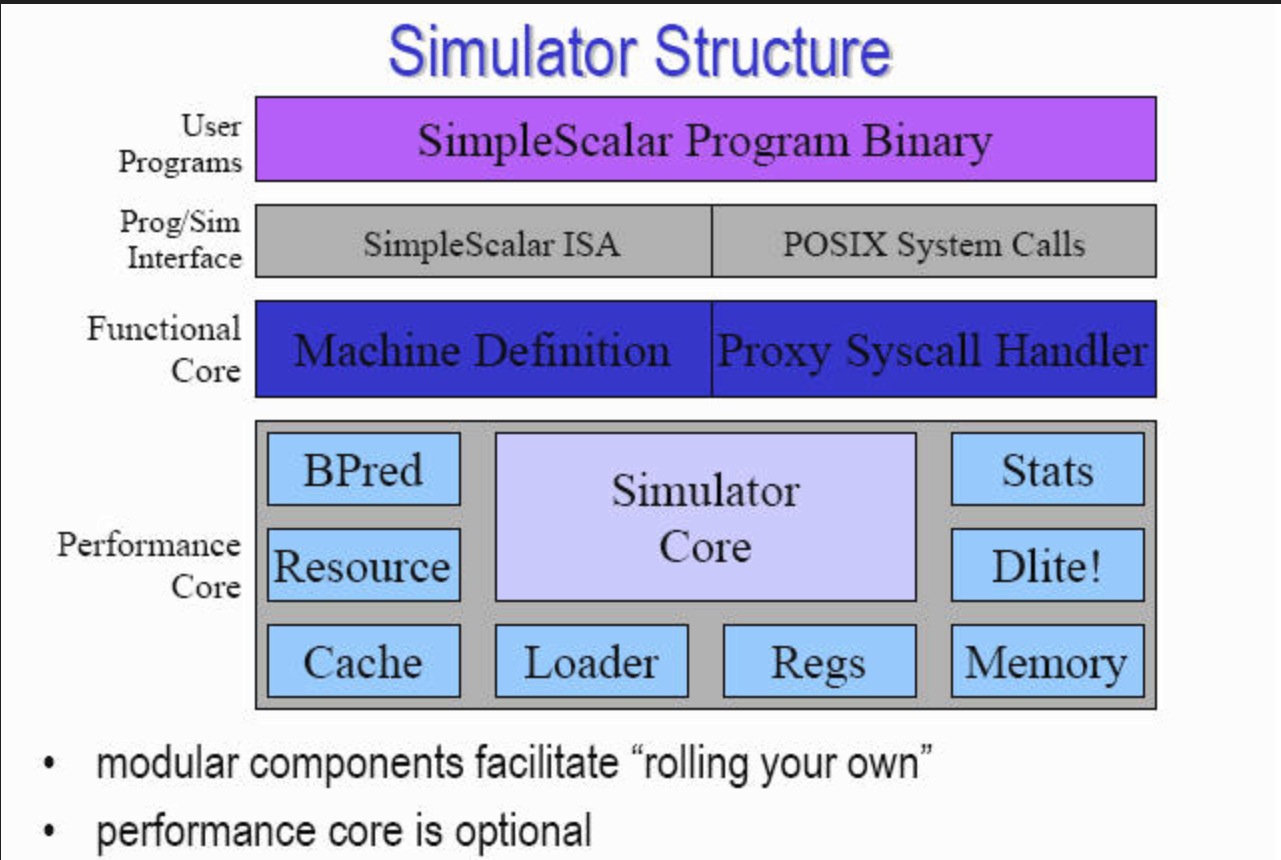
\includegraphics[width=0.75\linewidth]{images/simple-sim.png}
\caption{Arhitectura SimpleScalar}
\label{fig:simple-sim}
\end{figure}

% -------------------------------------------------- OGEHL
\subsection{Predictorul de ramificatii OGEHL}
\label{sec:ogehl}

\textbf{OGEHL} (Optimized Geometric History Length predictor) este un predictor
de ramificatii modern care foloseste mai multe tabele de predictie, fiecare
indexat cu o fereastra de istorie globala de lungime diferita. Lungimile
sunt dispuse geometric, ceea ce permite capturarea atat a corelatiilor scurte,
cat si a celor lungi din comportamentul branch-urilor. Contributiile fiecarui
tabel sunt sumate, iar semnul sumei finale determina decizia de predictie
(\textit{taken} / \textit{not taken}). Predictorul include mecanisme adaptive
pentru ajustarea pragului de decizie si a lungimii istoriei utilizate.

% -------------------------------------------------- Wang '97
\subsection{Predictorul de valori Wang '97}
\label{sec:wang}

\textbf{Wang~'97 hybrid value predictor} este un predictor de valori propus de
Wang si Franklin in 1997. Acesta combina mai multi predictori simpli (de tip
\textit{last-value} si \textit{stride}) si foloseste un mecanism de selectie
dinamica pentru a alege predictia cea mai probabila pentru valoarea rezultatului
unei instructiuni. Scopul sau este reducerea dependentelor de date prin
speculatie asupra valorilor, nu asupra fluxului de control.

% -------------------------------------------------- Comparatie
\subsection{OGEHL vs Wang~'97}
\label{sec:comparatie}

Desi ambii predictori sunt sisteme hibride bazate pe exploatarea istoricului
executiei, ei opereaza in domenii fundamental diferite ale procesorului:

\begin{itemize}
    \item \textbf{OGEHL} lucreaza pe \textit{control flow prediction}:
          foloseste istoricul branch-urilor pentru a prezice directia de salt.
          Spatiul de predictie este binar (\textit{taken} / \textit{not taken}).
    \item \textbf{Wang~'97} lucreaza pe \textit{data value prediction}:
          incearca sa anticipeze direct valoarea numerica produsa de o
          instructiune aritmetica sau de load/store, un spatiu de predictie
          mult mai larg si mai variabil.
\end{itemize}

La nivel de mecanism, OGEHL agrega contributiile mai multor tabele intr-un
singur scor de decizie printr-o suma cu actualizare adaptiva, in timp ce
Wang~'97 foloseste un \textit{meta-selector} care alege explicit intre
predictori specializati. Diferenta esentiala este ca OGEHL optimizeaza
corectitudinea fluxului de executie (\textit{control dependencies}), in timp
ce Wang~'97 incearca sa reduca latenta prin specularea valorilor
(\textit{data dependencies}), ceea ce implica un cost de risc si o
complexitate mai ridicate in practica.

% -------------------------------------------------- Hardware
\subsection{Arhitectura Hardware OGEHL}
\label{sec:hw}

Predictorul OGEHL este compus din patru componente hardware principale care
interactioneaza intr-un pipeline de predictie si actualizare.

\subsubsection*{Componentele hardware}

\begin{itemize}
    \item \textbf{Tabele de predictie} --- Un set de $N$ tabele, fiecare
          continand contoare saturate pe $k$ biti. La predictie, fiecare
          tabel $i$ este indexat cu o functie derivata din PC-ul instructiunii
          si din primii $L[i]$ biti ai GHR (XOR intre PC si fereastra de
          istorie). Valoarea contorului accesat este adaugata la suma globala.

    \item \textbf{Contoare saturate} --- Folosite in trei roluri distincte:
          \begin{enumerate}
              \item \textit{Contoarele de predictie} din tabele ($k$ biti,
                    implicit 4), care codifica tendinta locala a unui branch;
              \item \textit{Aliasing counter} (9 biti), care monitorizeaza
                    rata de aliasing in tabelul dinamic si decide daca se
                    foloseste o istorie lunga sau scurta a GHR-ului;
              \item \textit{Threshold counter} (7 biti), care controleaza
                    actualizarea dinamica a pragului de decizie $\theta$.
          \end{enumerate}

    \item \textbf{Global History Register (GHR)} --- Un registru de
          deplasare pe 32 de biti care retine istoricul global al
          rezultatelor branch-urilor recente. La fiecare branch rezolvat,
          GHR este deplasat la stanga cu 1 bit si se insereaza rezultatul
          real (\textit{taken} = 1, \textit{not taken} = 0). Lungimea
          efectiva de istorie utilizata pentru tabelul $i$ este:
          $$L[i] = \left\lfloor \alpha^{\,i-1} \cdot L_1 + 0.5 \right\rfloor$$
          unde $\alpha = 2$ si $L_1 = 2$ sunt parametri implicitii.

    \item \textbf{Sumator} --- Agrega contributiile tuturor tabelelor
          intr-o singura valoare intreaga \textit{sum}. Decizia de predictie
          este \textit{taken} daca $\mathit{sum} \geq 0$, respectiv
          \textit{not taken} in caz contrar. Suma este utilizata si in
          logica de actualizare: contoarele sunt actualizate doar la
          mispredictie sau cand $|\mathit{sum}| \leq \theta$, evitand
          actualizarile inutile pe predictii corecte si sigure.
\end{itemize}

\subsubsection*{Fluxul de functionare}

\paragraph{Predictie.}
Pentru un PC dat, fiecare tabel $i$ calculeaza un index:
\[
  \mathit{idx}_i = \bigl(PC \oplus \mathit{GHR}[0:L[i]]\bigr) \bmod \mathit{tableSize}
\]
Contorul de la acel index este citit si adaugat la suma globala. Semnul sumei
finale produce decizia binara.

\paragraph{Actualizare.}
Dupa rezolvarea branch-ului, predictorul executa trei operatii in ordine:

\begin{enumerate}
    \item \textbf{Actualizarea contoarelor de predictie}: daca a existat
          mispredictie sau $|\mathit{sum}| \leq \theta$, fiecare contor
          accesat este incrementat (branch \textit{taken}) sau decrementat
          (branch \textit{not taken}).

    \item \textbf{Ajustarea dinamica a lungimii istoriei}
          (\textit{Dynamic History Length Fitting}): aliasing counter-ul
          detecteaza daca mispredictiile recente sunt cauzate de aliasing
          in tabelul dinamic (tabelul 6). Daca aliasing counter-ul
          satureaza pozitiv, se comuta la un GHR mai lung pentru tabelele
          cu indici pari; daca satureaza negativ, se revine la GHR scurt.

    \item \textbf{Ajustarea adaptiva a pragului $\theta$}
          (\textit{Adaptive Threshold Fitting}): threshold counter-ul este
          incrementat la mispredictie si decrementat cand predictia este
          corecta dar $|\mathit{sum}| \leq \theta$. La saturare, valoarea
          $\theta$ este ajustata in sus sau in jos, adaptand sensibilitatea
          predictorului la comportamentul curent al programului.
\end{enumerate}

\subsubsection*{Parametrii predictorului}

Implementarea expune trei parametri configurabili, prezentati in
Tabelul~\ref{tab:params}.

\begin{table}[H]
    \centering
    \small
    \begin{tabular}{|l|c|c|c|l|}
        \hline
        \textbf{Parametru} & \textbf{Implicit} & \textbf{Min} & \textbf{Max} & \textbf{Descriere} \\
        \hline
        Numar de tabele ($N$)      & 7    & 4 & 12    & Numarul de tabele de predictie \\
        Marimea tabelelor          & 2048 & 1 & 88000 & Numarul de intrari per tabel \\
        Lungimea contoarelor ($k$) & 4    & 3 & 5     & Precizia contoarelor saturate (biti) \\
        \hline
        $\alpha$ (raport geometric) & 2   & -- & --   & Factorul de crestere al istoriei \\
        $L_1$ (istorie minima)      & 2   & -- & --   & Lungimea istoriei pentru tabelul 1 \\
        $\theta$ initial            & $N$ & -- & --   & Pragul adaptiv de actualizare \\
        \hline
    \end{tabular}
    \caption{Parametrii predictorului OGEHL}
    \label{tab:params}
\end{table}

\begin{figure}[H]
	\centering
	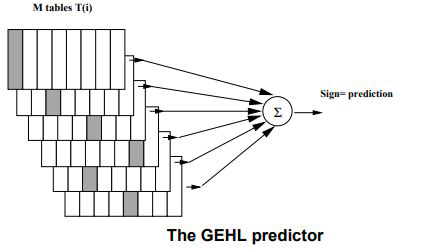
\includegraphics[width=0.75\linewidth]{images/oghel.png}
	\caption{Structura hardware OGEHL}
	\label{fig:oghel}
\end{figure}
